\documentclass[11pt]{article}

\usepackage[margin=1in]{geometry}
\usepackage{graphicx}
\usepackage{booktabs}
\usepackage{hyperref}
\usepackage{natbib}
\usepackage{siunitx}
\usepackage{xcolor}
\usepackage{microtype}
\usepackage{enumitem}
\usepackage{etoolbox}
\usepackage{array}
\usepackage{amsmath}
\usepackage{amssymb}

\AtBeginEnvironment{thebibliography}{\sloppy}
\setlength{\emergencystretch}{1em}

\title{Memory Dominates Routing: A Controlled Screening \\
of Neuroscience-Inspired Transformer Blocks}
\author{Riyad Mehdiyev}
\date{March 2026}

\begin{document}
\maketitle

% ==================================================================
%  ABSTRACT
% ==================================================================
\begin{abstract}
The best combination of three neuroscience-inspired
blocks---surprise-gated routing, episodic working memory, and homeostatic
normalization---reduces validation loss from 6.30 to 2.72 on GSM8K when added
to a frozen 360M-parameter transformer with LoRA, a 57\% relative improvement
over the LoRA-only baseline.
This result emerged from a controlled screening sweep: we proposed six
architectural modules motivated by predictive processing, complementary learning
systems, adaptive control, and homeostatic regulation, then tested four of them
on SmolLM-360M with LoRA adaptation (100 steps, TPU~v4).
The sweep reveals a clear hierarchy.
Episodic memory~(B2) combined with homeostatic normalization~(B6) is the
dominant factor.
A surprise gate~(B1) adds a gain only when memory is also
present---unexpectedly, B1 \emph{hurts} when paired with B6 alone (2.99 vs.\
2.74), suggesting its value lies in directing tokens toward memory operations.
A per-layer critic~(B3) degrades every configuration it enters.
Two further blocks---predictive coding~(B4) and an RL gating
policy~(B5)---were deferred on theoretical grounds before screening began.
These results reduce a broad six-block hypothesis space to two
high-confidence candidates for second-stage evaluation at scale.
\end{abstract}

% ==================================================================
%  INTRODUCTION
% ==================================================================
\section{Introduction}

\begin{figure}[t]
  \centering
  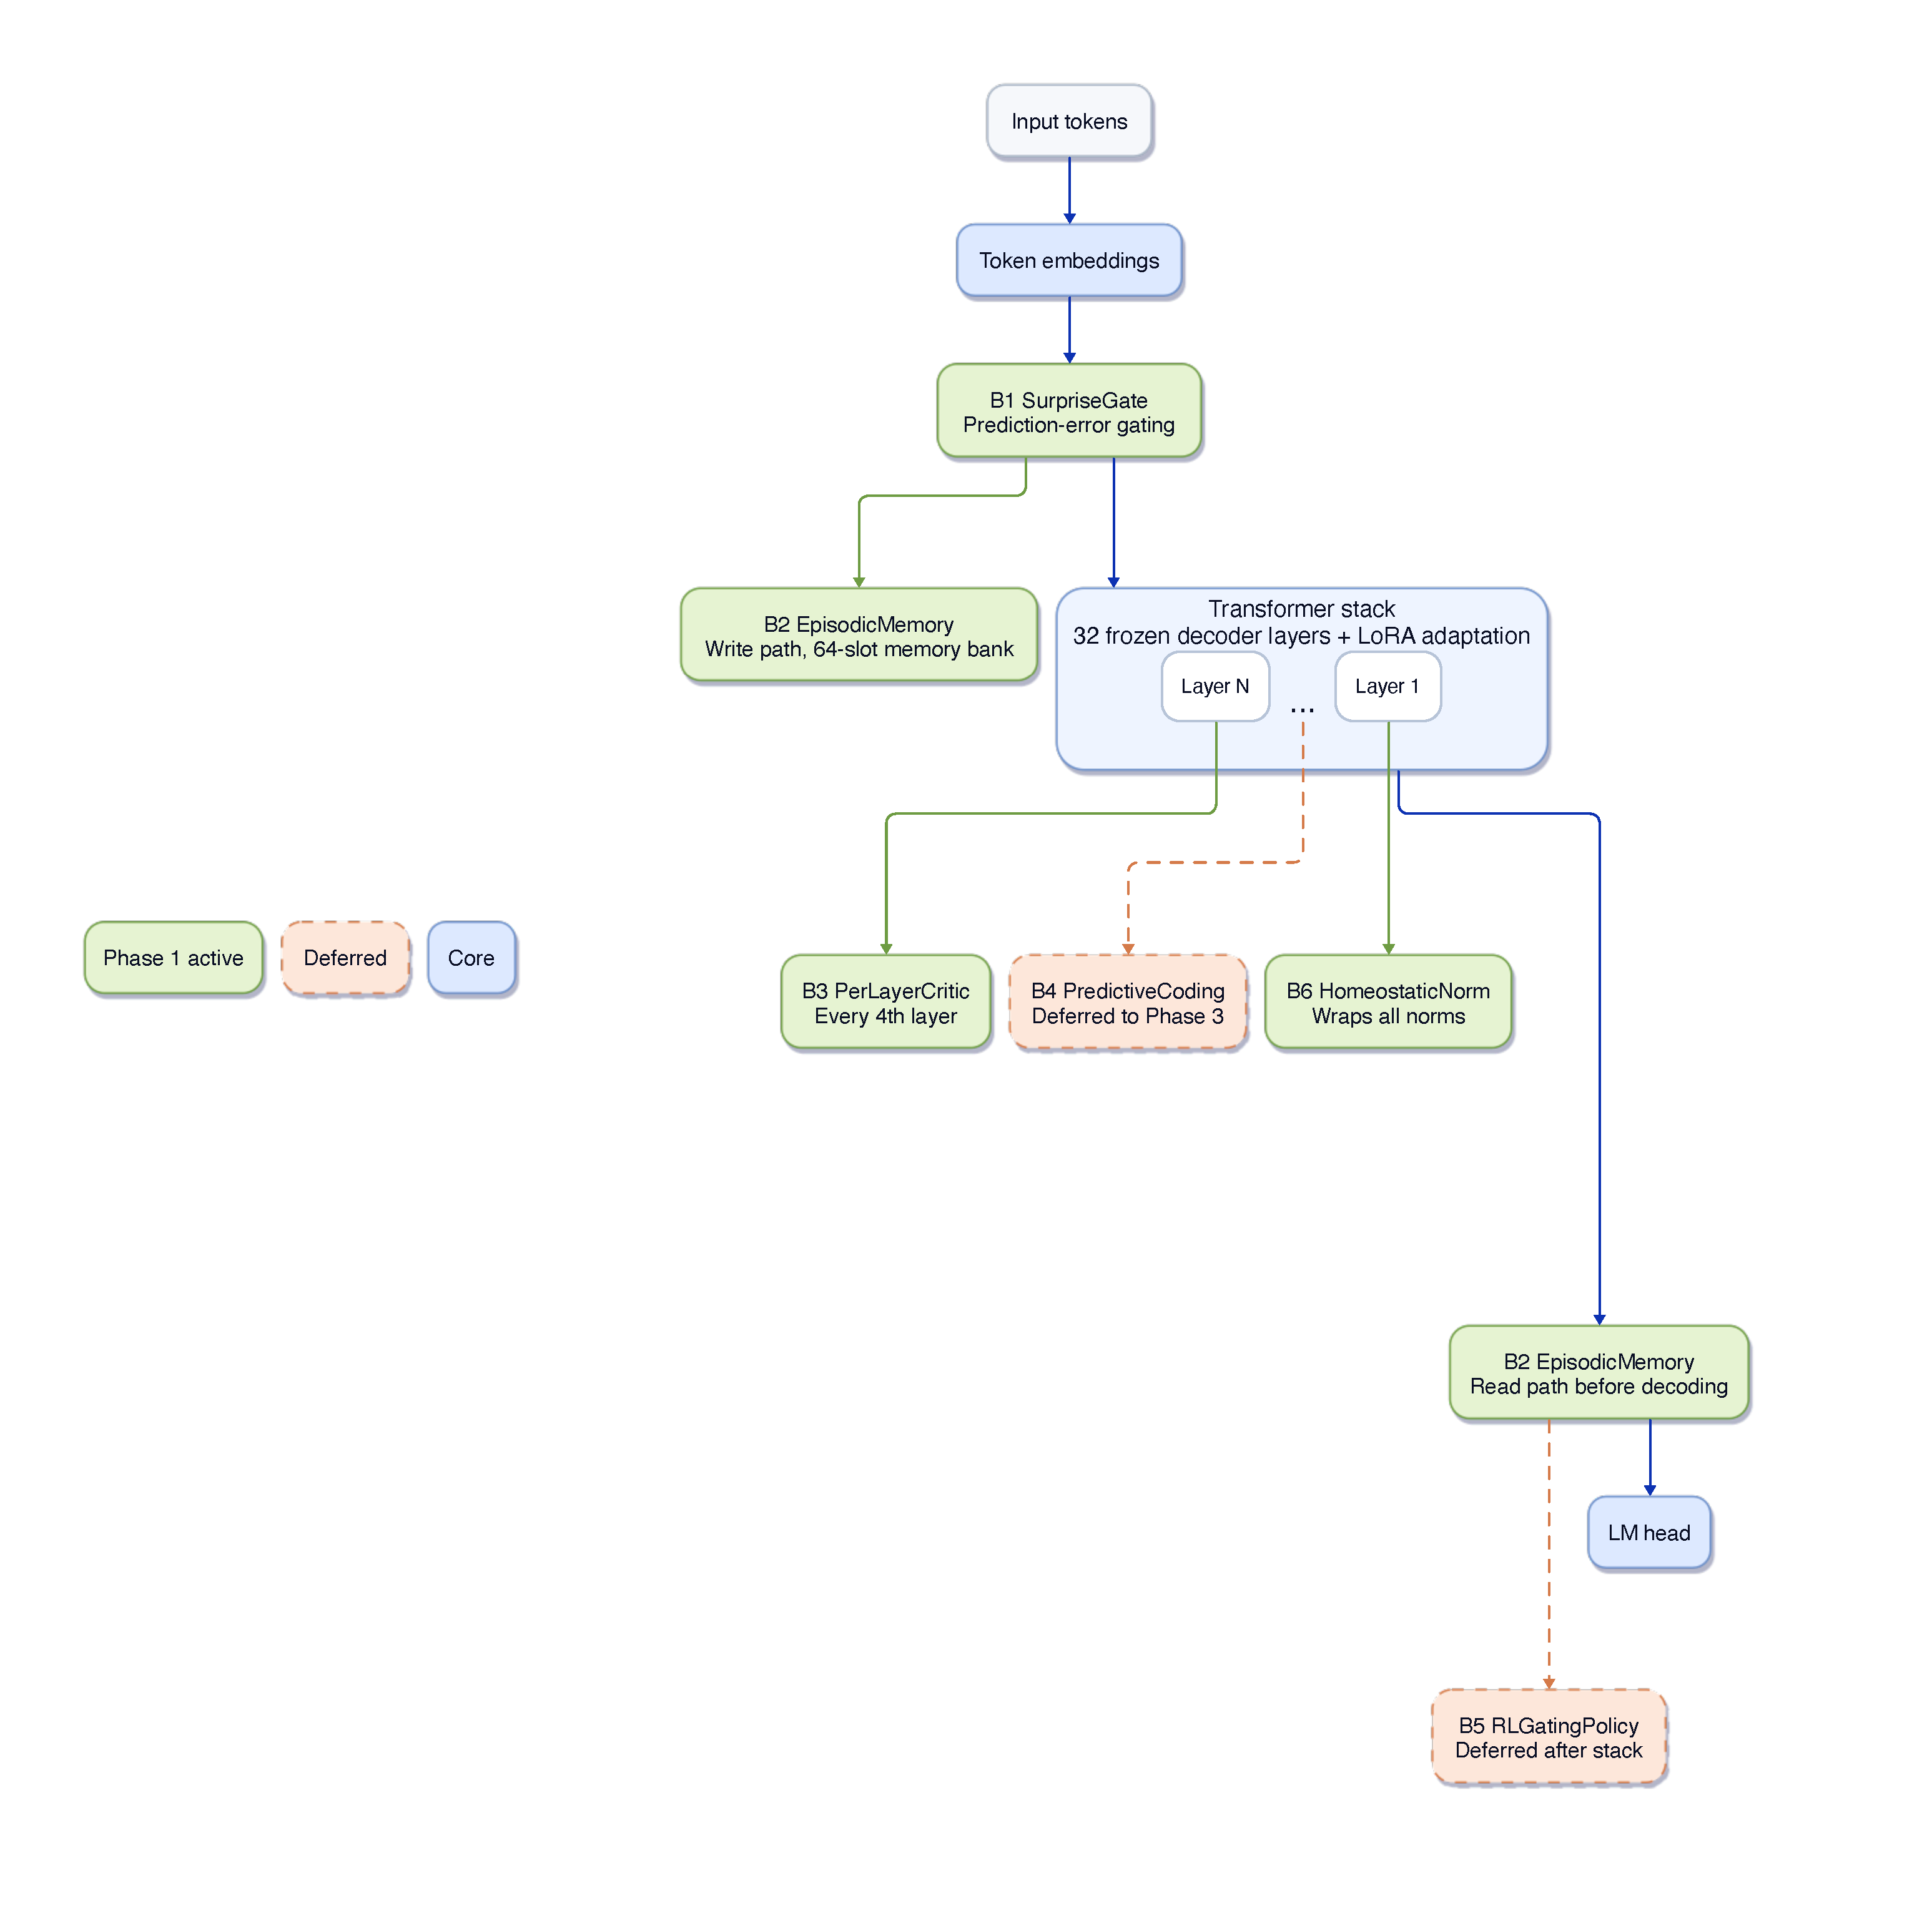
\includegraphics[width=\linewidth]{figures/architecture_overview.pdf}
  \caption{Architecture overview.  Green blocks were screened in Phase~1;
  orange blocks were deferred.  Among the screened blocks, B1, B2, and B6
  are promoted to Phase~2 candidates; B3 is eliminated.}
  \label{fig:architecture}
\end{figure}

Modern language-model papers frequently borrow motivation from neuroscience, yet
most such links remain metaphorical \citep{hassabis2017neuroscience}.
We take a more concrete approach: define explicit modules corresponding to
specific neuroscience-inspired hypotheses, insert them into a transformer, and
evaluate them through controlled ablations.

Our architecture adds six candidate blocks to a causal decoder transformer,
each targeting a different design question: adaptive routing, working memory,
depth-distributed credit assignment, predictive coding, learned orchestration,
and homeostatic stabilization.
Claiming that all six matter without empirical screening would be premature.
We therefore screen four of them under a tight 100-step TPU budget.
The screen produces a clear ranking: \textbf{episodic memory and homeostatic
normalization account for nearly all of the observed gain}, while
surprise-gated routing adds a small complement and a per-layer critic
consistently underperforms.

Perhaps the most striking finding is that homeostatic normalization
alone---a modification adding only 125K trainable parameters---accounts for
the majority of the improvement.
This suggests that the primary bottleneck for augmenting small frozen
transformers with new modules is not the sophistication of those modules but
the stability of the training process that integrates them.

\paragraph{Contributions.}
\begin{enumerate}[leftmargin=1.5em]
  \item A six-block neuroscience-inspired transformer extension covering
        adaptive routing, working memory, credit assignment, predictive coding,
        learned orchestration, and homeostatic stabilization
        (Section~\ref{sec:method}).
  \item A controlled screening protocol---analogous to successive-halving model
        selection \citep{li2018hyperband}---that ranks block combinations under
        a fixed 100-step TPU budget, enabling cheap elimination of weak
        candidates (Section~\ref{sec:setup}).
  \item Evidence that memory and stabilization dominate the design space:
        B2+B6 and B1+B2+B6 reduce validation loss by ${\approx}57\%$, while
        B3-containing variants trail by 10+ percentage points
        (Section~\ref{sec:results}).
  \item A principled reduction from six blocks to two high-confidence
        candidates for second-stage evaluation
        (Section~\ref{sec:discussion}).
\end{enumerate}

% ==================================================================
%  RELATED WORK
% ==================================================================
\section{Related Work}

\paragraph{Neuroscience-inspired AI.}
High-level arguments for importing neuroscience principles into AI are well
developed \citep{hassabis2017neuroscience}.
We are closest in spirit to that agenda but more concrete: rather than drawing
broad inspiration from memory, prediction, and control, we implement explicit
modules and evaluate them empirically.

\paragraph{Adaptive computation and routing.}
The idea of input-dependent computation depth traces to adaptive computation
time \citep{graves2016act}.
More recent work includes Mixture-of-Depths \citep{raposo2024mod} and Inner
Thinking Transformer \citep{itt2025}, both showing that token-dependent routing
is a productive engineering direction.
B1's distinctive claim is not that adaptive routing is new, but that a
surprise-motivated signal may be a useful way to structure it.

\paragraph{Memory augmentation.}
B2 is closest to episodic-memory language-model work \citep{emllm2025}.
The critical difference is scale: we test a small, explicit module under a cheap
screening protocol rather than claiming a mature long-context memory system.

\paragraph{Normalization and training stability.}
B6 relates to the broader normalization literature
\citep{ba2016layernorm,zhang2019rmsnorm}.
The key distinction is that B6 tracks a running exponential moving average of
activation variance across training steps, providing an inertial stabilizer
against the distribution shift introduced by LoRA parameter updates---rather
than normalizing only within a single forward pass.

\paragraph{Auxiliary losses and deep supervision.}
B3 connects to deep supervision \citep{lee2015deeply} and auxiliary-loss
training, though our formulation uses TD-style bootstrapping across depth
rather than direct supervision at intermediate layers.

\medskip\noindent
The gap our screening fills is empirical: while each of these ideas has been
studied in isolation, no prior work has systematically compared their
contributions within a single architecture under controlled conditions.

% ==================================================================
%  METHOD
% ==================================================================
\section{Method}
\label{sec:method}

\subsection{Base Transformer and Modification Strategy}

We start from a standard causal decoder transformer with hidden dimension
$d = 960$ (SmolLM-360M, 32 layers, 15 attention heads) and insert or wrap
additional modules at specific points in the computation graph
(Figure~\ref{fig:architecture}).
The wrapper model:
\begin{itemize}[leftmargin=1.5em]
  \item inserts B1 immediately after token embeddings,
  \item writes to and reads from B2 around the transformer stack,
  \item attaches B3 value heads at every 4th layer,
  \item inserts B4 between layers (deferred to Phase~2),
  \item places B5 after the stack as a controller (deferred to Phase~2),
  \item and replaces all normalization layers with B6.
\end{itemize}

\subsection{Block Definitions}

Table~\ref{tab:block-overview} summarizes the six blocks.
Each corresponds to a specific architectural hypothesis.

\begin{table}[t]
\centering
\small
\begin{tabular}{>{\raggedright\arraybackslash}p{0.06\linewidth}
                >{\raggedright\arraybackslash}p{0.16\linewidth}
                >{\raggedright\arraybackslash}p{0.22\linewidth}
                >{\raggedright\arraybackslash}p{0.20\linewidth}
                >{\raggedright\arraybackslash}p{0.22\linewidth}}
\toprule
Block & Name & Placement & Hypothesis & Status \\
\midrule
B1 & SurpriseGate & After embeddings & Should difficult tokens receive adaptive computation? & Screened \\
B2 & EpisodicMemory & Write before / read after stack & Can explicit working memory help a small LM? & Screened \\
B3 & PerLayerCritic & Every 4th layer & Does intermediate credit assignment improve optimization? & Screened \\
B4 & PredictiveCoding & Between layers & Can error-driven inter-layer processing help? & Deferred \\
B5 & RLGatingPolicy & After stack & Should a learned controller orchestrate blocks? & Deferred \\
B6 & HomeostaticNorm & Replaces all norms & Do these perturbations need explicit stabilization? & Screened \\
\bottomrule
\end{tabular}
\caption{The six candidate blocks, their architectural hypotheses,
and Phase-1 screening status.}
\label{tab:block-overview}
\end{table}

\paragraph{B1: SurpriseGate.}
B1 computes a token-level surprise signal.
An exponential moving average~(EMA) tracks the batch-mean hidden state with
decay $\tau = 0.99$:
\[
\bar{h} \leftarrow \tau\,\bar{h}
  + (1 - \tau)\,\frac{1}{BS}\sum_{b,s} h_{b,s}.
\]
This is a \emph{global} prior---deliberately collapsing batch and sequence
dimensions so that the surprise signal reflects deviation from the overall
distribution rather than position-specific expectations.
A single-layer prior network $p\colon \mathbb{R}^d \to \mathbb{R}^d$ predicts
the current hidden state from this running average.
The surprise score is the sigmoid output of a two-layer MLP
($d \to 64 \to 1$) applied to the prediction error:
\[
s_t = \sigma\!\bigl(\mathrm{MLP}(h_t - p(\bar{h}))\bigr) \in [0,1].
\]
The score is discretized into $K{=}3$ depth buckets via learnable thresholds
$\theta_1, \theta_2$ initialized at 0.3 and 0.7.
Tokens in deeper buckets receive full-depth processing; shallow-bucket tokens
may skip later layers.
B1 contributes an auxiliary prediction loss
$L_{\mathrm{B1}} = \mathrm{MSE}\!\bigl(p(h_{1:T-1}),\, h_{2:T}\bigr)$
scaled by $\lambda_1 = 0.01$.

\paragraph{B2: EpisodicMemory.}
B2 maintains $M{=}64$ key--value memory slots.
Let $K \in \mathbb{R}^{M \times d}$ denote the learnable keys (initialized
from $\mathcal{N}(0,0.02)$) and $V \in \mathbb{R}^{M \times d}$ the value
buffer.

\emph{Write.}\; A gated update determines how strongly each token writes:
\[
g_t = \sigma(W_g\, h_t + b_g), \qquad b_g \text{ initialized to } {-}2.0,
\]
yielding an initial gate of ${\approx}0.12$---deliberately conservative so
that writes remain small early in training.
Attention weights $a = \mathrm{softmax}(h_t\, K^\top)$ distribute the gated
write across slots; slot updates blend the new write with the previous value
via a learnable per-slot gate.

\emph{Read.}\; Queries and keys are projected to a 128-dimensional bottleneck
before computing scaled dot-product attention over the value buffer:
\[
\hat{h}_t = h_t + \sigma(\alpha)\;
  W_o\;\mathrm{softmax}\!\!\left(\frac{W_q h_t\,(W_k K)^\top}{\sqrt{128}}\right) V,
\]
where $W_o$ is \emph{zero-initialized} so that B2 starts as an identity and
gradually learns to contribute.
B2 adds no auxiliary loss; its effect is purely through the forward-pass
modification.

\paragraph{B3: PerLayerCritic.}
B3 attaches a value head (Linear--GELU--LayerNorm--Linear, hidden dim 256) at
every 4th transformer layer (8 heads total for 32 layers).
Each head predicts a scalar value from the sequence-mean-pooled hidden state.
The auxiliary loss uses a temporal-difference~(TD) target bootstrapped backward
through depth:
\[
L_{\mathrm{B3}} = \sum_l \mathrm{MSE}\!\left(V_l,\;
  \mathcal{L}_{\mathrm{LM}} + \gamma\, V_{l+1}\right),
  \quad \gamma = 0.95,
\]
where $V_L$ at the deepest critic bootstraps directly from the language-model
loss $\mathcal{L}_{\mathrm{LM}}$.
The discount $\gamma = 0.95$ follows standard RL convention; we did not tune
this value.
As Section~\ref{sec:results} shows, this formulation did not improve
optimization under the 100-step budget.

\paragraph{B4 and B5 (deferred).}
B4 (PredictiveCoding) inserts a predictor between layers and emphasizes the
residual between predicted and observed activations, approximating a
predictive-processing hierarchy \citep{rao1999predictive}.
B5~(RLGatingPolicy) is a policy head mapping hidden states to one of four
actions (pass, write-memory, deepen-compute, recall-memory).
Both were deferred; see Section~\ref{sec:scope} for the rationale.

\paragraph{B6: HomeostaticNorm.}
B6 wraps all normalization layers (LayerNorm or RMSNorm, 65 total) and tracks
running activation statistics via an EMA with decay $\tau = 0.99$.
The output is:
\[
\mathrm{B6}(x) = \mathrm{BaseNorm}(x) \cdot (\gamma_{\mathrm{adapt}} \cdot c)
  + \beta_{\mathrm{adapt}},
  \quad
  c = \mathrm{clamp}\!\left(\frac{1}{\sqrt{\mathrm{Var}_{\mathrm{EMA}}
  + \epsilon}},\; 0.1,\; 10\right),
\]
where $\gamma_{\mathrm{adapt}}$ and $\beta_{\mathrm{adapt}}$ are learned
per-dimension scale and bias.
This provides an inertial stabilizer analogous to homeostatic synaptic scaling
in biological neural circuits: the system resists chronic over- or
under-excitation regardless of what other blocks are active.
B6 adds no auxiliary loss.

We note that B6's practical value may be largely an engineering contribution
(adaptive normalization for LoRA-adapted models) rather than evidence for
homeostatic plasticity as a computational principle.
Disentangling these interpretations requires comparing against
non-neuroscience-motivated adaptive normalization baselines in Phase~2.

\subsection{Training Objective}

The total loss combines the language-model cross-entropy with auxiliary block
losses:
\[
L_{\mathrm{total}} = \mathcal{L}_{\mathrm{LM}}
  + \lambda_1\, L_{\mathrm{B1}}
  + \lambda_3\, L_{\mathrm{B3}},
\]
where $\lambda_1 = 0.01$ and $\lambda_3 = 0.1$.
B2 and B6 contribute no auxiliary loss.
When a block is disabled for ablation, its $\lambda$ term is zeroed.

\begin{table}[t]
\centering
\small
\begin{tabular}{lrrl}
\toprule
Component & Added params & \% of base & Notes \\
\midrule
B1 (SurpriseGate) & 983K & 0.27\% & Dominated by prior network ($d^2$) \\
B2 (EpisodicMemory) & 1.23M & 0.34\% & Dominated by memory projection ($d^2$) \\
B3 (PerLayerCritic, $\times$8) & 1.97M & 0.54\% & 8 heads across 32 layers \\
B6 (HomeostaticNorm, $\times$65) & 125K & 0.03\% & Scale + bias per norm layer \\
\midrule
LoRA (rank 16, Q/V only) & 1.97M & 0.54\% & 32 layers $\times$ 2 projections \\
\bottomrule
\end{tabular}
\caption{Parameter overhead of each screened block relative to the
362M-parameter base model.  B1 and B2 each add roughly half the parameters of
LoRA; B3 matches LoRA in count.  Only B6 is negligible in size.}
\label{tab:param-overhead}
\end{table}

% ==================================================================
%  EXPERIMENTAL SETUP
% ==================================================================
\section{Experimental Setup}
\label{sec:setup}

\subsection{Screening Protocol}

We screened each configuration using:
\begin{itemize}[leftmargin=1.5em]
  \item Base model: SmolLM-360M \citep{smollm360m,smollm3blog2025} (frozen)
  \item Adaptation: LoRA \citep{hu2022lora} (rank 16, $\alpha{=}32$,
        dropout 0.05) on all query and value projections
  \item Dataset: GSM8K training split \citep{cobbe2021gsm8k}
  \item Hardware: non-spot Cloud TPU~v4
  \item Budget: 100 AdamW steps ($\beta_1{=}0.9$, $\beta_2{=}0.999$, weight
        decay $0.01$, lr $2{\times}10^{-4}$, linear warmup over 10 steps)
  \item Batch size: 4
  \item Validation: loss on a capped 64-example subset
  \item Primary metric: validation loss
  \item Total sweep wall time: ${\approx}$45 minutes (8 configs, 4--6 min each)
\end{itemize}

We deliberately omitted generation-based GSM8K accuracy: the objective was to
rank configurations cheaply, not to establish final reasoning performance.

\subsection{Scope: Why Four of Six Blocks}
\label{sec:scope}

The screening protocol must decide which blocks are ready to test.
B1, B2, B3, and B6 entered the sweep; B4 and B5 were deferred before any
screening data was collected:
\begin{itemize}[leftmargin=1.5em]
  \item B4's implementation does not faithfully realize top-down predictive
        coding and remained unstable in preliminary runs.
  \item B5 requires a training regime long enough for a policy to learn
        meaningful orchestration; 100 steps is insufficient.
\end{itemize}
Deferring known-unstable blocks prevents contamination of the sweep and is a
deliberate part of the protocol design.

\subsection{Pre-Study Hypotheses}

Before running the sweep, we predicted:
\begin{enumerate}[leftmargin=1.5em]
  \item B2+B6 would be strongest (memory + stability).
  \item B6 alone would give the safest standalone gain.
  \item B1 would likely help, especially paired with B2.
  \item B3 would contribute less than memory-centered variants.
\end{enumerate}

\subsection{Screened Configurations}

The sweep consisted of one LoRA-only baseline and seven block configurations,
covering all subsets of $\{$B1, B2, B3$\} \times \{$B6$\}$:

\begin{center}
\small
LoRA only \quad|\quad B6 \quad|\quad B1+B6 \quad|\quad B2+B6 \quad|\quad
B3+B6 \quad|\quad B1+B2+B6 \quad|\quad B2+B3+B6 \quad|\quad B1+B2+B3+B6
\end{center}

\begin{table}[t]
\centering
\small
\begin{tabular}{lrr}
\toprule
Configuration & Val.\ loss & Reduction (\%) \\
\midrule
\textbf{B1+B2+B6} & \textbf{2.718} & \textbf{56.85} \\
\textbf{B2+B6} & \textbf{2.722} & \textbf{56.79} \\
B6 & 2.743 & 56.45 \\
B1+B6 & 2.990 & 52.53 \\
\midrule
B1+B2+B3+B6 & 3.451 & 45.21 \\
B2+B3+B6 & 3.493 & 44.54 \\
B3+B6 & 3.572 & 43.29 \\
\midrule
LoRA only (baseline) & 6.299 & --- \\
\bottomrule
\end{tabular}
\caption{Phase-1 screening results, sorted by validation loss (best first).
Base model: SmolLM-360M (frozen) + LoRA rank~16.
Metric: validation loss on a 64-example GSM8K subset after 100 AdamW steps on
TPU~v4 (lower is better).
Reduction is relative to the LoRA-only baseline.
Bold marks the top-tier configurations (within 0.01 of each other).
All results are single runs without confidence intervals.}
\label{tab:phase1-results}
\end{table}


% ==================================================================
%  RESULTS
% ==================================================================
\section{Results}
\label{sec:results}

All results are single-run evaluations on a 64-example validation subset.
We report these as a \emph{ranking screen}, not as statistically confirmed
effects.
Configurations separated by fewer than 0.1 loss points should be treated as
tied at the resolution of this protocol.
Table~\ref{tab:phase1-results} reports the complete sweep and
Figure~\ref{fig:ranking} visualizes the ranking.

\begin{figure}[t]
  \centering
  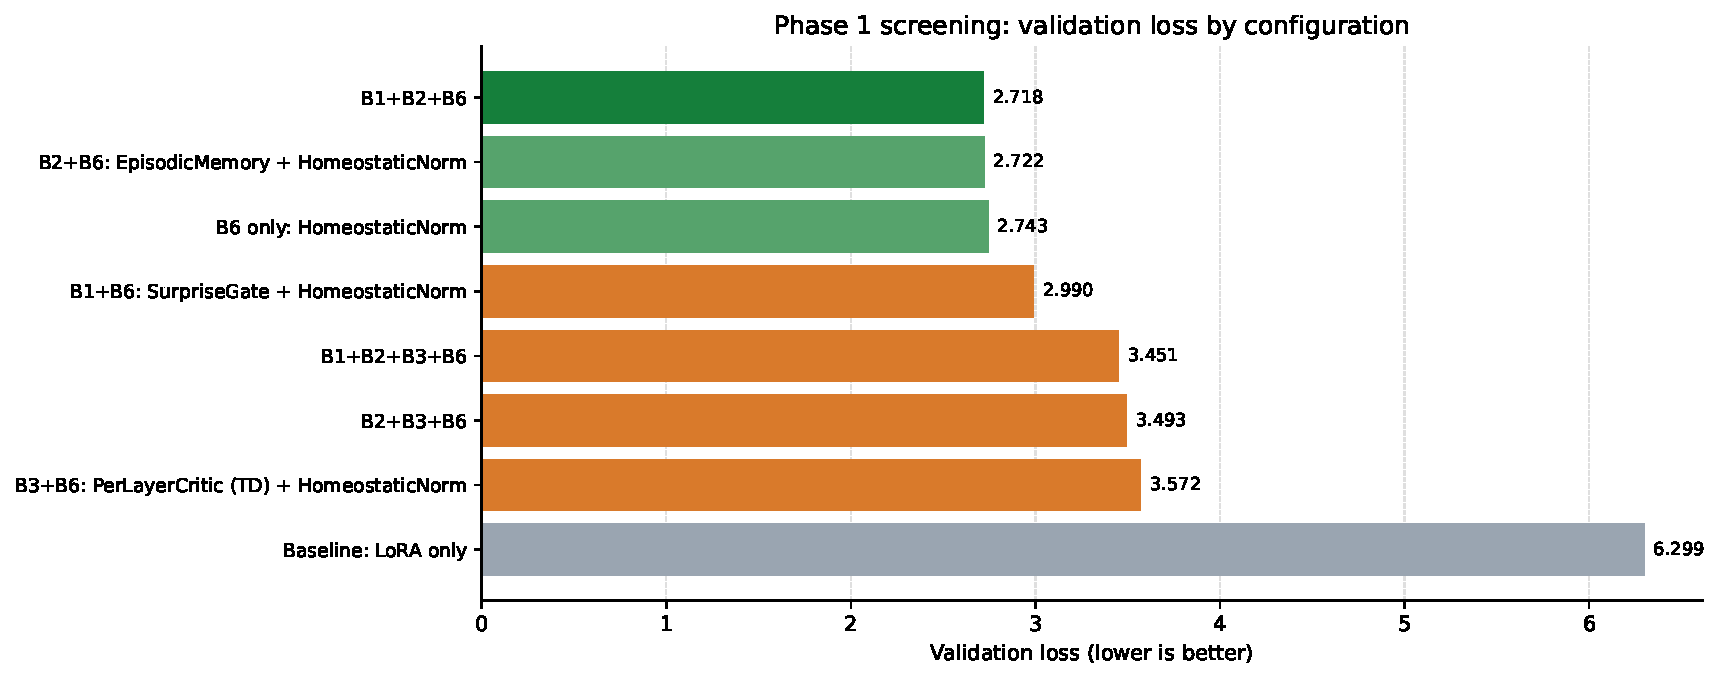
\includegraphics[width=\linewidth]{figures/phase1_val_loss_ranking.pdf}
  \caption{Validation-loss ranking for the Phase-1 screening sweep (lower is
  better).  Configurations within 0.1 of the best should be treated as tied
  under the single-run protocol.}
  \label{fig:ranking}
\end{figure}

\paragraph{Top tier: memory + stabilization.}
The two strongest configurations were B1+B2+B6 (validation loss 2.718) and
B2+B6 (2.722).
Their 0.004 difference is well within the noise floor of a single run on 64
examples; we treat them as tied.
Both share episodic memory and homeostatic normalization, suggesting that this
pairing is the primary driver.

\paragraph{Homeostatic normalization alone.}
B6 alone reached 2.743---a 56.4\% improvement over the LoRA-only baseline
(6.299) from a block with only 125K parameters.
This was the most surprising result in the sweep and confirms B6 as the safest
single-block addition.

\paragraph{B1 hurts without B2.}
B1+B6 reached 2.990, \emph{worse} than B6 alone (2.743).
Adding surprise-gated routing without episodic memory appears to disrupt the
forward pass without providing compensating information flow.
B1's benefit appeared only when B2 was also present (B1+B2+B6: 2.718 vs.\
B2+B6: 2.722), suggesting that surprise routing helps primarily by directing
tokens toward memory read/write operations.
This interaction is one of the more informative findings of the sweep.

\paragraph{Per-layer critic: negative result.}
Every B3-containing configuration trailed the best memory-centered variants:
B3+B6 (3.572), B2+B3+B6 (3.493), B1+B2+B3+B6 (3.451).
B3's TD-bootstrapped loss likely requires many more steps to stabilize than the
forward-pass losses used by B1 and B2, making the 100-step budget particularly
unfavorable.
The current formulation does not merit inclusion in Phase~2 without redesign.

\paragraph{Summary ranking.}
\begin{center}
B1+B2+B6 $\approx$ B2+B6 $\gtrsim$ B6 $>$ B1+B6
$\gg$ B1+B2+B3+B6 $\gtrsim$ B2+B3+B6 $\gtrsim$ B3+B6
\end{center}

\paragraph{Baseline calibration.}
The LoRA-only baseline (6.299) was substantially higher than all B6-enhanced
configurations ($\leq$2.99).
We verified that the baseline used the same learning rate, warmup, and data
pipeline.
The large gap likely reflects the difficulty of fine-tuning a frozen 360M model
on mathematical reasoning with only LoRA and standard LayerNorm: without B6's
adaptive variance tracking, the optimizer must simultaneously learn the task
\emph{and} compensate for the distribution shift between frozen and adapted
representations.
This interpretation is testable in Phase~2 by comparing LoRA+B6 against full
fine-tuning without B6.

\paragraph{Parameter confound.}
The corrected parameter counts (Table~\ref{tab:param-overhead}) reveal that B1
and B2 each add roughly half as many parameters as LoRA, and B3 matches LoRA in
count.
The observed gains therefore cannot be attributed purely to block
\emph{mechanisms}---they may partly reflect additional trainable capacity.
B6, with only 125K parameters, is the one block whose gains are unlikely to be
explained by capacity alone.
A parameter-matched random baseline (see Section~\ref{sec:limitations}) is
essential for Phase~2.

% ==================================================================
%  DISCUSSION
% ==================================================================
\section{Discussion}
\label{sec:discussion}

The screening narrows the original six-block proposal to a focused
two-candidate design.

\paragraph{Stabilization is the dominant effect.}
B6 alone accounts for most of the improvement.
We hypothesize that LoRA adaptation of a frozen model creates a distribution
shift in activation statistics that standard LayerNorm does not track across
training steps.
B6's EMA-based correction acts as an implicit learning-rate adaptation that
stabilizes the interaction between frozen weights and trainable LoRA parameters.
This is consistent with the observation that \emph{all} strong configurations
include B6.
Disentangling the stabilization benefit from a genuine ``homeostatic''
contribution requires comparing against other adaptive normalization baselines
in Phase~2.

\paragraph{Memory adds a real but modest gain.}
B2+B6 matched the best three-block configuration within noise.
The marginal contribution of episodic memory over stabilization alone is smaller
than our pre-study hypothesis predicted, but it is consistent across
configurations: B2+B6 $<$ B6 by 0.02, and adding B2 to B1+B6 (2.990
$\to$ 2.718 via B1+B2+B6) produced the largest single-block marginal gain in
the sweep.

\paragraph{Routing needs memory to help.}
The B1+B6 $>$ B6 reversal (where adding B1 \emph{increased} loss) is the most
informative interaction effect.
It suggests that surprise-gated depth routing is only useful when there is a
downstream consumer of the routing signal---in this case, the memory read/write
system.
Without B2, the routing simply adds noise to the forward pass.

\paragraph{Comparison to pre-study hypotheses.}
Predictions were largely confirmed: B2+B6 is among the strongest
(prediction~1), B6 alone is the safest addition (prediction~2), and B3 is the
weakest (prediction~4).
The partial surprise is that B6 alone nearly matches B2+B6, and that B1 hurts
without B2---neither was anticipated.

% ==================================================================
%  LIMITATIONS
% ==================================================================
\section{Limitations}
\label{sec:limitations}

\paragraph{Short-budget regime.}
Each configuration received only 100 optimization steps---enough to identify a
broad ranking but not to establish convergence or to fairly evaluate blocks
(like B3) whose auxiliary losses require many steps to stabilize.

\paragraph{Single metric.}
Validation loss was the only screening metric.
This is appropriate for a cheap screen but insufficient for a final
reasoning-ability claim.

\paragraph{Single model size.}
Results are tied to SmolLM-360M.
Whether these effects survive at larger scale is the central question for
Phase~2.

\paragraph{No variance estimate.}
The sweep provides no multi-seed confidence intervals.
Configurations within 0.1 loss points cannot be reliably distinguished.

\paragraph{No parameter-matched control.}
We did not test a randomly initialized module with the same parameter count as
B2 (${\approx}$1.2M).
Such a control would isolate the benefit of the episodic-memory
\emph{mechanism} from the benefit of extra capacity.
Given the corrected parameter counts (Table~\ref{tab:param-overhead}), this
control is essential for Phase~2.

\paragraph{Incomplete B3 diagnosis.}
The screening reveals that B3 is the weakest block but cannot determine whether
this reflects a fundamental problem with depth-distributed credit assignment or
an implementation mismatch.
The TD-bootstrapped loss requires value heads to converge before providing
useful gradients---a chicken-and-egg problem exacerbated by a 100-step budget.
A fair evaluation would require a longer training horizon or a redesigned loss
that avoids bootstrapping.

\paragraph{No learning curves.}
We report only final validation loss at step 100.
Intermediate training curves would reveal whether B3's poor performance
reflects slower convergence (potentially recoverable) or a worse asymptote
(fundamental).
We recommend logging intermediate losses in Phase~2.

% ==================================================================
%  CONCLUSION
% ==================================================================
\section{Conclusion}

The screening reduces a six-block hypothesis space to two high-confidence
candidates: B2+B6 and B1+B2+B6.
The most actionable finding is about training stability: homeostatic
normalization alone recovers most of the available gain, suggesting that the
primary bottleneck for augmenting frozen transformers is not architectural
sophistication but the stability of the fine-tuning process.

Phase~2 should therefore:
(1)~build around B2+B6 as the core configuration;
(2)~test whether B1 adds a real incremental gain at larger scale;
(3)~include a parameter-matched random baseline to isolate mechanism from
capacity;
(4)~run multi-seed experiments with learning curves to establish confidence
intervals.
B3 should return only after replacing TD bootstrapping with a loss that
converges within feasible budgets.
B4 and B5 remain outside the evaluation path until their theoretical and
implementation gaps are closed.

% ==================================================================
%  ETHICS AND BROADER IMPACT
% ==================================================================
\section*{Ethics and Broader Impact}

This work proposes architectural modifications to a small, openly licensed
language model (SmolLM-360M, Apache 2.0) and does not involve human subjects,
private data, or deployment of generated text.
The screening protocol is designed to reduce wasted compute by eliminating
unpromising directions early---the entire sweep consumed approximately 45
minutes of TPU~v4 time.
We see no specific ethical concerns beyond those inherent to language-model
research generally.

\bibliographystyle{plainnat}
\bibliography{references}

\end{document}
